\documentclass{standalone}
\usepackage{tikz}
\begin{document}
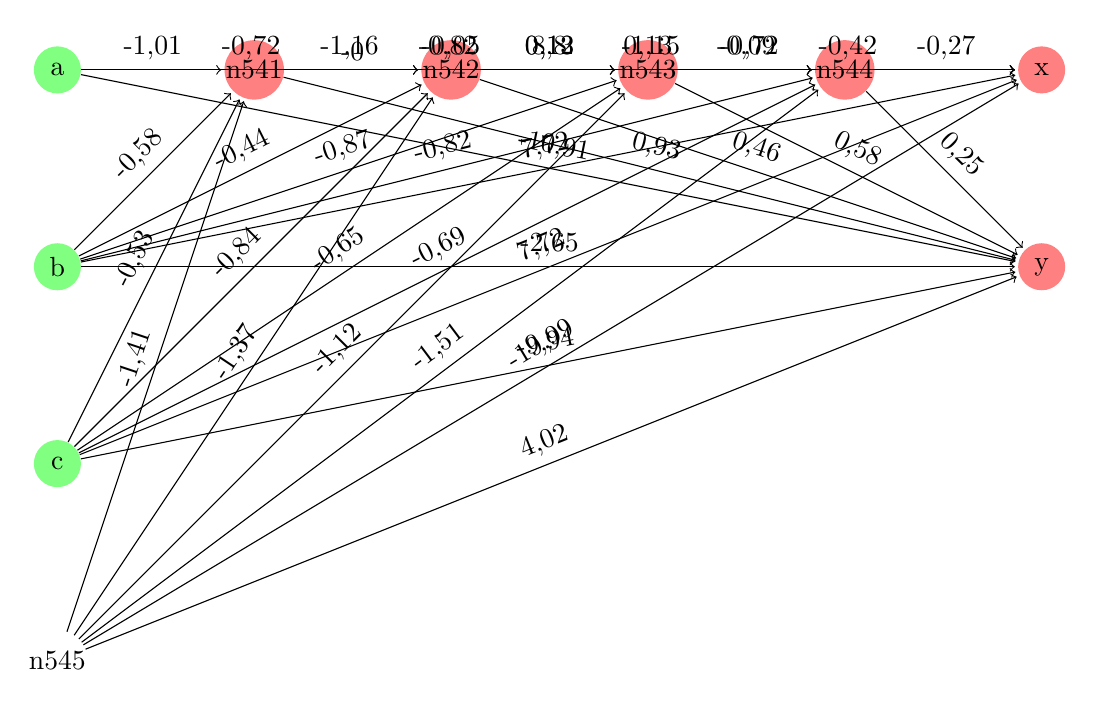
\begin{tikzpicture}[shorten >=1pt,->,draw=black!,node distance=2.5cm]
\tikzstyle{neuron}=[circle,fill=black!25,minimum size=17pt,inner sep=0pt]
\tikzstyle{constant}=[neuron, fill=white!50];
\tikzstyle{sigmoid}=[neuron, fill=red!50];
\tikzstyle{identity}=[neuron, fill=green!50];
\node [identity] (a) {a};
\node [identity,below of=a] (b) {b};
\node [identity,below of=b] (c) {c};
\node [constant,below of=c] (n545) {n545};
\node [sigmoid,right of=a] (n541) {n541};
\node [sigmoid,right of=n541] (n542) {n542};
\node [sigmoid,right of=n542] (n543) {n543};
\node [sigmoid,right of=n543] (n544) {n544};
\node [sigmoid,right of=n544] (x) {x};
\node [sigmoid,below of=x] (y) {y};
\path[every node/.style={sloped,anchor=south,auto=false}]
(n542) edge node {0,46} (y)
(n542) edge node {-0,72} (x)
(n542) edge node {0,13} (n544)
(n542) edge node {0,12} (n543)
(c) edge node {7,72} (x)
(c) edge node {-9,94} (y)
(c) edge node {-0,53} (n541)
(c) edge node {-0,84} (n542)
(c) edge node {-0,65} (n543)
(c) edge node {-0,69} (n544)
(n541) edge node {-1,15} (x)
(n541) edge node {0,93} (y)
(n541) edge node {-0,05} (n543)
(n541) edge node {-0} (n542)
(n541) edge node {0,13} (n544)
(n544) edge node {0,25} (y)
(n544) edge node {-0,27} (x)
(n543) edge node {-0,42} (x)
(n543) edge node {0,58} (y)
(n543) edge node {-0,09} (n544)
(n545) edge node {-19,99} (x)
(n545) edge node {-1,41} (n541)
(n545) edge node {4,02} (y)
(n545) edge node {-1,12} (n543)
(n545) edge node {-1,37} (n542)
(n545) edge node {-1,51} (n544)
(b) edge node {7,72} (x)
(b) edge node {-2,65} (y)
(b) edge node {-0,58} (n541)
(b) edge node {-0,44} (n542)
(b) edge node {-0,87} (n543)
(b) edge node {-0,82} (n544)
(a) edge node {8,8} (x)
(a) edge node {-0,82} (n544)
(a) edge node {-10,91} (y)
(a) edge node {-1,01} (n541)
(a) edge node {-0,72} (n542)
(a) edge node {-1,16} (n543)
;\end{tikzpicture}
\end{document}